% ===========================================================================
%  TikuOS — TikuKits DS: Stack for Embedded Systems
%  Beamer Presentation
% ===========================================================================
\documentclass[aspectratio=169, 10pt]{beamer}

% ---- Theme ----------------------------------------------------------------
\usetheme{Madrid}
\usecolortheme{whale}
\setbeamertemplate{navigation symbols}{}
\setbeamertemplate{footline}{%
  \leavevmode\hbox{%
    \begin{beamercolorbox}[wd=.33\paperwidth,ht=2.5ex,dp=1ex,center]{author in head/foot}%
      \usebeamerfont{author in head/foot}\insertshortauthor
    \end{beamercolorbox}%
    \begin{beamercolorbox}[wd=.34\paperwidth,ht=2.5ex,dp=1ex,center]{title in head/foot}%
      \usebeamerfont{title in head/foot}\insertshorttitle
    \end{beamercolorbox}%
    \begin{beamercolorbox}[wd=.33\paperwidth,ht=2.5ex,dp=1ex,right]{date in head/foot}%
      \usebeamerfont{date in head/foot}\insertshortdate{}\hspace*{2em}%
      \insertframenumber{}/\inserttotalframenumber\hspace*{2ex}
    \end{beamercolorbox}}%
  \vskip0pt%
}

% ---- Packages -------------------------------------------------------------
\usepackage{listings}
\usepackage{graphicx}
\usepackage{hyperref}
\usepackage{booktabs}
\usepackage{multirow}
\usepackage{tikz}
\usetikzlibrary{arrows.meta, positioning, shapes.geometric, calc,
                decorations.pathreplacing, fit}
\usepackage{amsmath}

% ---- Code listing style ---------------------------------------------------
\lstset{
  basicstyle=\ttfamily\scriptsize,
  keywordstyle=\color{blue}\bfseries,
  commentstyle=\color{gray},
  stringstyle=\color{red!70!black},
  showstringspaces=false,
  breaklines=true,
  frame=single,
  rulecolor=\color{black!30},
  backgroundcolor=\color{blue!3},
  tabsize=4,
}
\lstdefinestyle{cstyle}{
  language=C,
  morekeywords={uint8_t,uint16_t,uint32_t,int32_t,int16_t,
                tiku_kits_ds_elem_t,
                TIKU_KITS_DS_OK,TIKU_KITS_DS_ERR_NULL,
                TIKU_KITS_DS_ERR_FULL,TIKU_KITS_DS_ERR_EMPTY,
                TIKU_KITS_DS_ERR_PARAM,TIKU_KITS_DS_ERR_NOTFOUND,
                TIKU_KITS_DS_ERR_BOUNDS,
                TIKU_KITS_DS_STACK_MAX_SIZE,
                NULL},
}

% ---- Metadata -------------------------------------------------------------
\title[TikuKits DS]{TikuKits DS: Stack for Embedded Systems}
\subtitle{Simple. Ubiquitous. Intelligence, Everywhere.}
\author[Ambuj Varshney]{Ambuj Varshney \\ \texttt{ambuj@tiku-os.org}}
\date{\today}

% ===========================================================================
\begin{document}

% ---------------------------------------------------------------------------
\begin{frame}
\titlepage
\end{frame}

% ---------------------------------------------------------------------------
\begin{frame}{Outline}
\tableofcontents
\end{frame}

% ===========================================================================
\section{Motivation}
% ===========================================================================

\begin{frame}{Why a Stack on MCUs?}
\begin{columns}[T]
\begin{column}{0.48\textwidth}
\begin{block}{Embedded Use Cases}
\begin{itemize}
  \item \textbf{Balanced bracket parsing} --- validate protocol frames
  \item \textbf{Undo/redo operations} --- reverse the last N actions
  \item \textbf{DFS traversal} --- iterative depth-first search on graphs
  \item \textbf{Expression evaluation} --- postfix / RPN calculators
  \item \textbf{State save/restore} --- push context, pop on return
\end{itemize}
\end{block}

\begin{block}{Constraints}
\begin{itemize}
  \item No heap allocation
  \item Fixed, bounded memory usage
  \item $O(1)$ push and pop
  \item Deterministic worst-case behavior
\end{itemize}
\end{block}
\end{column}

\begin{column}{0.48\textwidth}
\begin{center}
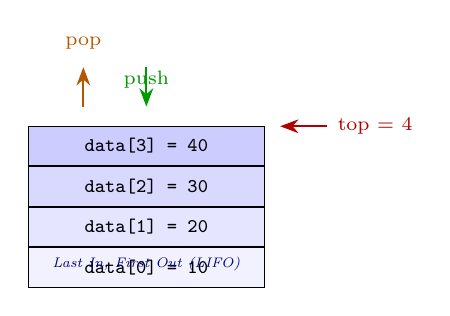
\begin{tikzpicture}[>=Stealth, node distance=0.15cm]
  % Stack visualization (vertical)
  \node[draw, minimum width=3cm, minimum height=0.5cm,
        fill=blue!20, font=\scriptsize\ttfamily] (s3) {data[3] = 40};
  \node[draw, minimum width=3cm, minimum height=0.5cm,
        fill=blue!15, font=\scriptsize\ttfamily, below=0cm of s3] (s2) {data[2] = 30};
  \node[draw, minimum width=3cm, minimum height=0.5cm,
        fill=blue!10, font=\scriptsize\ttfamily, below=0cm of s2] (s1) {data[1] = 20};
  \node[draw, minimum width=3cm, minimum height=0.5cm,
        fill=blue!5, font=\scriptsize\ttfamily, below=0cm of s1] (s0) {data[0] = 10};

  % Top pointer
  \draw[->, thick, red!70!black] (2.3, 0.25) -- (1.7, 0.25)
    node[right=0.6cm, font=\scriptsize] {top = 4};

  % Push/Pop arrows
  \draw[->, thick, green!60!black] (0, 1.0) -- (0, 0.5)
    node[above=0.1cm, font=\scriptsize] {push};
  \draw[->, thick, orange!70!black] (-0.8, 0.5) -- (-0.8, 1.0)
    node[above=0.1cm, font=\scriptsize] {pop};

  % LIFO label
  \node[font=\tiny\itshape, text=blue!50!black] at (0, -1.5)
    {Last In, First Out (LIFO)};
\end{tikzpicture}
\end{center}

\vspace{0.3em}
\begin{alertblock}{Design Goal}
Provide a fixed-size LIFO stack with $O(1)$ push, pop, and peek,
\textbf{zero heap usage}, and safe overflow/underflow detection.
\end{alertblock}
\end{column}
\end{columns}
\end{frame}

% ===========================================================================
\section{Data Structure}
% ===========================================================================

\begin{frame}[fragile]{The \texttt{tiku\_kits\_ds\_stack} Structure}
\begin{columns}[T]
\begin{column}{0.48\textwidth}
\begin{lstlisting}[style=cstyle,
  title={ds/stack/tiku\_kits\_ds\_stack.h}]
#ifndef TIKU_KITS_DS_STACK_MAX_SIZE
#define TIKU_KITS_DS_STACK_MAX_SIZE 16
#endif

struct tiku_kits_ds_stack {
    tiku_kits_ds_elem_t
        data[TIKU_KITS_DS_STACK_MAX_SIZE];
    uint16_t top;       /* next write pos */
    uint16_t capacity;  /* user limit     */
};
\end{lstlisting}

\vspace{0.3em}
\textbf{Memory footprint:}\\
$16 \times 4 + 2 + 2 = 68$ bytes (default).\\
All statically allocated --- no heap.
\end{column}

\begin{column}{0.48\textwidth}
\textbf{Top pointer semantics:}
\begin{center}
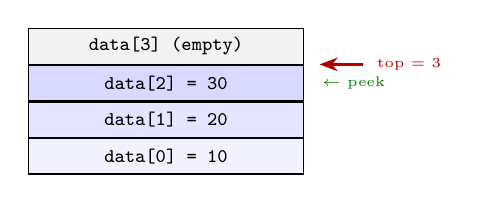
\begin{tikzpicture}[>=Stealth, node distance=0.0cm]
  \node[draw, minimum width=3.5cm, minimum height=0.45cm,
        fill=gray!10, font=\scriptsize\ttfamily] (e3) {data[3] (empty)};
  \node[draw, minimum width=3.5cm, minimum height=0.45cm,
        fill=blue!15, font=\scriptsize\ttfamily, below=0cm of e3] (e2) {data[2] = 30};
  \node[draw, minimum width=3.5cm, minimum height=0.45cm,
        fill=blue!10, font=\scriptsize\ttfamily, below=0cm of e2] (e1) {data[1] = 20};
  \node[draw, minimum width=3.5cm, minimum height=0.45cm,
        fill=blue!5, font=\scriptsize\ttfamily, below=0cm of e1] (e0) {data[0] = 10};

  \draw[->, thick, red!70!black] (2.5, -0.23) -- (1.95, -0.23)
    node[right=0.6cm, font=\tiny] {top = 3};

  \node[font=\tiny, right=0.1cm of e2, text=green!50!black] {$\leftarrow$ peek};
\end{tikzpicture}
\end{center}

\vspace{0.5em}
\begin{block}{Key Properties}
\begin{itemize}
  \item \texttt{top = 0}: stack is empty
  \item \texttt{top = capacity}: stack is full
  \item Push writes \texttt{data[top++]}
  \item Pop reads \texttt{data[--top]}
  \item Peek reads \texttt{data[top - 1]}
\end{itemize}
\end{block}
\end{column}
\end{columns}
\end{frame}

% ===========================================================================
\section{API Reference}
% ===========================================================================

\begin{frame}[fragile]{Complete API}
\begin{table}
\centering
\small
\begin{tabular}{@{}lp{8cm}@{}}
\toprule
\textbf{Function} & \textbf{Description} \\
\midrule
\texttt{\_stack\_init(stk, cap)}
  & Initialize with capacity $1 \ldots$ \texttt{MAX\_SIZE}; zeros data \\
\texttt{\_stack\_push(stk, val)}
  & Write at \texttt{data[top]}, increment top; returns \texttt{ERR\_FULL} \\
\texttt{\_stack\_pop(stk, \&val)}
  & Decrement top, read \texttt{data[top]}; returns \texttt{ERR\_EMPTY} \\
\texttt{\_stack\_peek(stk, \&val)}
  & Read \texttt{data[top - 1]} without removing \\
\midrule
\texttt{\_stack\_clear(stk)}
  & Reset top to 0 \\
\texttt{\_stack\_size(stk)}
  & Return current number of elements (== top) \\
\texttt{\_stack\_full(stk)}
  & Return 1 if top $\geq$ capacity \\
\texttt{\_stack\_empty(stk)}
  & Return 1 if top $= 0$ \\
\bottomrule
\end{tabular}
\end{table}

\vspace{0.3em}
{\scriptsize All functions are prefixed with \texttt{tiku\_kits\_ds}.
Every function validates pointer arguments and returns \texttt{ERR\_NULL} on failure.}

\begin{alertblock}{Overflow and Underflow Protection}
\texttt{push()} returns \texttt{ERR\_FULL} when the stack is at capacity.
\texttt{pop()} returns \texttt{ERR\_EMPTY} when the stack is empty.
No silent corruption.
\end{alertblock}
\end{frame}

% ===========================================================================
\section{How It Works}
% ===========================================================================

\begin{frame}[fragile]{Push and Pop Implementation}
\begin{columns}[T]
\begin{column}{0.48\textwidth}
\begin{lstlisting}[style=cstyle,
  title={push --- write at top, increment}]
int tiku_kits_ds_stack_push(
    struct tiku_kits_ds_stack *stk,
    tiku_kits_ds_elem_t value)
{
    if (stk == NULL)
        return TIKU_KITS_DS_ERR_NULL;
    if (stk->top >= stk->capacity)
        return TIKU_KITS_DS_ERR_FULL;

    stk->data[stk->top] = value;
    stk->top++;
    return TIKU_KITS_DS_OK;
}
\end{lstlisting}

\vspace{0.3em}
\begin{block}{Push Sequence}
\begin{enumerate}
  \item Check not full
  \item Write value at \texttt{data[top]}
  \item Increment \texttt{top}
\end{enumerate}
\end{block}
\end{column}

\begin{column}{0.48\textwidth}
\begin{lstlisting}[style=cstyle,
  title={pop --- decrement top, read}]
int tiku_kits_ds_stack_pop(
    struct tiku_kits_ds_stack *stk,
    tiku_kits_ds_elem_t *value)
{
    if (stk == NULL || value == NULL)
        return TIKU_KITS_DS_ERR_NULL;
    if (stk->top == 0)
        return TIKU_KITS_DS_ERR_EMPTY;

    stk->top--;
    *value = stk->data[stk->top];
    return TIKU_KITS_DS_OK;
}
\end{lstlisting}

\vspace{0.3em}
\begin{block}{Pop Sequence}
\begin{enumerate}
  \item Check not empty
  \item Decrement \texttt{top}
  \item Read value from \texttt{data[top]}
\end{enumerate}
\end{block}
\end{column}
\end{columns}
\end{frame}

% ===========================================================================
\section{Code Examples}
% ===========================================================================

\begin{frame}[fragile]{Example 1: Basic Push, Pop, and Peek}
\begin{lstlisting}[style=cstyle,
  title={Basic stack operations}]
#include "tikukits/ds/stack/tiku_kits_ds_stack.h"

struct tiku_kits_ds_stack stk;
tiku_kits_ds_elem_t val;

/* Initialize with capacity 8 */
tiku_kits_ds_stack_init(&stk, 8);

/* Push three values */
tiku_kits_ds_stack_push(&stk, 10);
tiku_kits_ds_stack_push(&stk, 20);
tiku_kits_ds_stack_push(&stk, 30);
/* top == 3, size() returns 3 */

/* Peek reads the top without removing */
tiku_kits_ds_stack_peek(&stk, &val);      /* val == 30 */

/* Pop returns in LIFO order */
tiku_kits_ds_stack_pop(&stk, &val);       /* val == 30 */
tiku_kits_ds_stack_pop(&stk, &val);       /* val == 20 */
tiku_kits_ds_stack_pop(&stk, &val);       /* val == 10 */

/* Stack is now empty */
int rc = tiku_kits_ds_stack_pop(&stk, &val);
/* rc == TIKU_KITS_DS_ERR_EMPTY */
\end{lstlisting}
\end{frame}

% ---------------------------------------------------------------------------
\begin{frame}[fragile]{Example 2: Interleaved Push and Pop}
\begin{columns}[T]
\begin{column}{0.48\textwidth}
\begin{lstlisting}[style=cstyle,
  title={Interleaved operations}]
struct tiku_kits_ds_stack stk;
tiku_kits_ds_elem_t val;

tiku_kits_ds_stack_init(&stk, 8);

/* Push A, B */
tiku_kits_ds_stack_push(&stk, 100);
tiku_kits_ds_stack_push(&stk, 200);

/* Pop: returns 200 (LIFO) */
tiku_kits_ds_stack_pop(&stk, &val);
/* val == 200 */

/* Push C */
tiku_kits_ds_stack_push(&stk, 300);

/* Pop: returns 300 (newest) */
tiku_kits_ds_stack_pop(&stk, &val);
/* val == 300 */

/* Pop: returns 100 (oldest) */
tiku_kits_ds_stack_pop(&stk, &val);
/* val == 100 */
\end{lstlisting}
\end{column}

\begin{column}{0.48\textwidth}
\begin{center}
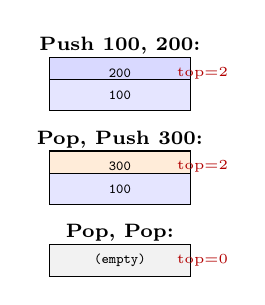
\begin{tikzpicture}[>=Stealth, scale=0.7]
  % Step 1
  \node[font=\scriptsize\bfseries] at (1.5, 4.2) {Push 100, 200:};
  \node[draw, minimum width=1.8cm, minimum height=0.4cm,
        fill=blue!15, font=\tiny\ttfamily] at (1.5, 3.7) {200};
  \node[draw, minimum width=1.8cm, minimum height=0.4cm,
        fill=blue!10, font=\tiny\ttfamily] at (1.5, 3.3) {100};
  \node[font=\tiny, red!70!black] at (3, 3.7) {top=2};

  % Step 2
  \node[font=\scriptsize\bfseries] at (1.5, 2.5) {Pop, Push 300:};
  \node[draw, minimum width=1.8cm, minimum height=0.4cm,
        fill=orange!15, font=\tiny\ttfamily] at (1.5, 2.0) {300};
  \node[draw, minimum width=1.8cm, minimum height=0.4cm,
        fill=blue!10, font=\tiny\ttfamily] at (1.5, 1.6) {100};
  \node[font=\tiny, red!70!black] at (3, 2.0) {top=2};

  % Step 3
  \node[font=\scriptsize\bfseries] at (1.5, 0.8) {Pop, Pop:};
  \node[draw, minimum width=1.8cm, minimum height=0.4cm,
        fill=gray!10, font=\tiny\ttfamily] at (1.5, 0.3) {(empty)};
  \node[font=\tiny, red!70!black] at (3, 0.3) {top=0};
\end{tikzpicture}
\end{center}

\vspace{0.3em}
\begin{block}{LIFO Guarantee}
Regardless of interleaving, the most recently
pushed element is always popped first.
\end{block}
\end{column}
\end{columns}
\end{frame}

% ===========================================================================
\section{Embedded Use Cases}
% ===========================================================================

\begin{frame}[fragile]{Use Case: Balanced Bracket Checker}
\begin{columns}[T]
\begin{column}{0.52\textwidth}
\begin{lstlisting}[style=cstyle,
  title={Validate bracket pairs in a protocol string}]
#include "tiku_kits_ds_stack.h"

/* Check if brackets in buf are balanced.
 * Supports (, ), [, ], curly braces.
 * Returns 1 if balanced, 0 otherwise. */
int brackets_balanced(const char *buf,
                      uint16_t len)
{
    struct tiku_kits_ds_stack stk;
    tiku_kits_ds_elem_t val;
    uint16_t i;

    tiku_kits_ds_stack_init(&stk, 16);

    for (i = 0; i < len; i++) {
        char ch = buf[i];
        if (ch == '(' || ch == '['
            || ch == '{') {
            if (tiku_kits_ds_stack_push(
                    &stk, (int32_t)ch)
                != TIKU_KITS_DS_OK)
                return 0;  /* overflow */
        } else if (ch == ')' || ch == ']'
                   || ch == '}') {
            if (tiku_kits_ds_stack_pop(
                    &stk, &val)
                != TIKU_KITS_DS_OK)
                return 0;  /* underflow */
            if (!is_matching(
                    (char)val, ch))
                return 0;  /* mismatch */
        }
    }
    return tiku_kits_ds_stack_empty(&stk);
}
\end{lstlisting}
\end{column}

\begin{column}{0.44\textwidth}
\begin{center}
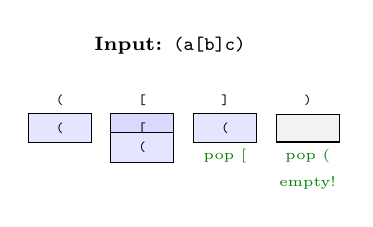
\begin{tikzpicture}[>=Stealth, scale=0.7]
  % Input string
  \node[font=\scriptsize\bfseries] at (2, 4.5) {Input: \texttt{(a[b]c)}};

  % Step-by-step stack states
  \node[font=\tiny\ttfamily] at (0, 3.5) {(};
  \node[draw, minimum width=0.8cm, minimum height=0.35cm,
        fill=blue!10, font=\tiny\ttfamily] at (0, 3.0) {(};

  \node[font=\tiny\ttfamily] at (1.5, 3.5) {[};
  \node[draw, minimum width=0.8cm, minimum height=0.35cm,
        fill=blue!15, font=\tiny\ttfamily] at (1.5, 3.0) {[};
  \node[draw, minimum width=0.8cm, minimum height=0.35cm,
        fill=blue!10, font=\tiny\ttfamily] at (1.5, 2.65) {(};

  \node[font=\tiny\ttfamily] at (3, 3.5) {]};
  \node[draw, minimum width=0.8cm, minimum height=0.35cm,
        fill=blue!10, font=\tiny\ttfamily] at (3, 3.0) {(};
  \node[font=\tiny, green!50!black] at (3, 2.5) {pop [};

  \node[font=\tiny\ttfamily] at (4.5, 3.5) {)};
  \node[draw, minimum width=0.8cm, minimum height=0.35cm,
        fill=gray!10, font=\tiny\ttfamily] at (4.5, 3.0) {};
  \node[font=\tiny, green!50!black] at (4.5, 2.5) {pop (};
  \node[font=\tiny, green!50!black] at (4.5, 2.0) {empty!};
\end{tikzpicture}
\end{center}

\vspace{0.5em}
\begin{block}{How It Works}
\begin{itemize}
  \item Push every opening bracket
  \item On closing bracket, pop and match
  \item At end, stack must be empty
  \item Stack capacity bounds nesting depth
\end{itemize}
\end{block}

\begin{alertblock}{Protocol Validation}
Useful for validating JSON-like config frames,
AT command responses, or nested protocol headers.
\end{alertblock}
\end{column}
\end{columns}
\end{frame}

% ---------------------------------------------------------------------------
\begin{frame}[fragile]{Use Case: DFS Traversal and State Save/Restore}
\begin{columns}[T]
\begin{column}{0.48\textwidth}
\begin{lstlisting}[style=cstyle,
  title={Iterative DFS using the stack}]
#include "tiku_kits_ds_stack.h"

/* Visit all reachable nodes from 'start'
 * in a graph stored as adjacency list */
void dfs_iterative(uint8_t start,
    const uint8_t adj[][MAX_NEIGHBORS],
    uint8_t visited[])
{
    struct tiku_kits_ds_stack stk;
    tiku_kits_ds_elem_t node;
    uint8_t i;

    tiku_kits_ds_stack_init(&stk, 16);
    tiku_kits_ds_stack_push(
        &stk, (int32_t)start);

    while (!tiku_kits_ds_stack_empty(&stk)) {
        tiku_kits_ds_stack_pop(&stk, &node);
        if (visited[(uint8_t)node])
            continue;
        visited[(uint8_t)node] = 1;
        process_node((uint8_t)node);

        for (i = 0; adj[(uint8_t)node][i]
             != 0xFF; i++) {
            tiku_kits_ds_stack_push(&stk,
                adj[(uint8_t)node][i]);
        }
    }
}
\end{lstlisting}
\end{column}

\begin{column}{0.48\textwidth}
\begin{lstlisting}[style=cstyle,
  title={State save/restore pattern}]
#include "tiku_kits_ds_stack.h"

static struct tiku_kits_ds_stack ctx_stack;

void context_init(void) {
    tiku_kits_ds_stack_init(&ctx_stack, 8);
}

/* Save current state before change */
void context_save(int32_t state) {
    tiku_kits_ds_stack_push(
        &ctx_stack, state);
}

/* Restore previous state (undo) */
int context_restore(int32_t *state) {
    if (tiku_kits_ds_stack_pop(
            &ctx_stack, state)
        == TIKU_KITS_DS_OK) {
        return 1;
    }
    return 0;  /* nothing to undo */
}
\end{lstlisting}

\vspace{0.3em}
\begin{block}{Bounded Undo}
Stack capacity limits undo depth ---
ideal for memory-constrained devices.
\end{block}
\end{column}
\end{columns}
\end{frame}

% ===========================================================================
\section{Memory Layout}
% ===========================================================================

\begin{frame}{Memory Layout and Sizing}
\begin{columns}[T]
\begin{column}{0.48\textwidth}
\begin{center}
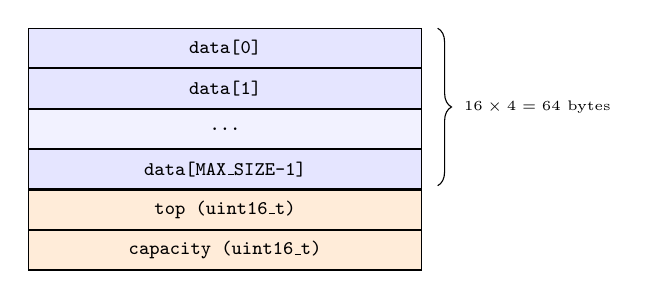
\begin{tikzpicture}[>=Stealth, node distance=0.0cm]
  \node[draw, minimum width=5cm, minimum height=0.5cm,
        fill=blue!10, font=\scriptsize\ttfamily] (d0) {data[0]};
  \node[draw, minimum width=5cm, minimum height=0.5cm,
        fill=blue!10, font=\scriptsize\ttfamily, below=0cm of d0] (d1) {data[1]};
  \node[draw, minimum width=5cm, minimum height=0.5cm,
        fill=blue!5, font=\scriptsize\ttfamily, below=0cm of d1] (d2) {...};
  \node[draw, minimum width=5cm, minimum height=0.5cm,
        fill=blue!10, font=\scriptsize\ttfamily, below=0cm of d2] (dn) {data[MAX\_SIZE-1]};
  \node[draw, minimum width=5cm, minimum height=0.5cm,
        fill=orange!15, font=\scriptsize\ttfamily, below=0cm of dn] (tp) {top (uint16\_t)};
  \node[draw, minimum width=5cm, minimum height=0.5cm,
        fill=orange!15, font=\scriptsize\ttfamily, below=0cm of tp] (cp) {capacity (uint16\_t)};

  \draw[decorate, decoration={brace, amplitude=5pt}]
    (2.7, 0.25) -- (2.7, -1.75)
    node[midway, right=6pt, font=\tiny] {$16 \times 4 = 64$ bytes};
\end{tikzpicture}
\end{center}
\end{column}

\begin{column}{0.48\textwidth}
\begin{block}{Size Formula}
\[
  \text{Total} = \texttt{MAX\_SIZE} \times \texttt{sizeof(elem\_t)} + 4
\]
\end{block}

\begin{table}
\centering
\scriptsize
\begin{tabular}{@{}rrr@{}}
\toprule
\textbf{MAX\_SIZE} & \textbf{elem\_t} & \textbf{Total (bytes)} \\
\midrule
4   & int32\_t & 20 \\
8   & int32\_t & 36 \\
16  & int32\_t & 68 \\
8   & int16\_t & 20 \\
16  & int16\_t & 36 \\
\bottomrule
\end{tabular}
\end{table}

\vspace{0.3em}
\begin{alertblock}{Minimal Overhead}
Only 4 bytes of metadata (top + capacity).
The simplest data structure in the DS library.
\end{alertblock}
\end{column}
\end{columns}
\end{frame}

% ===========================================================================
\section{Complexity}
% ===========================================================================

\begin{frame}{Time Complexity}
\begin{table}
\centering
\begin{tabular}{@{}lcc@{}}
\toprule
\textbf{Operation} & \textbf{Best Case} & \textbf{Worst Case} \\
\midrule
\texttt{init}   & $O(n)$ & $O(n)$ \\
\texttt{push}   & $O(1)$ & $O(1)$ \\
\texttt{pop}    & $O(1)$ & $O(1)$ \\
\texttt{peek}   & $O(1)$ & $O(1)$ \\
\texttt{clear}  & $O(1)$ & $O(1)$ \\
\texttt{size}   & $O(1)$ & $O(1)$ \\
\texttt{full}   & $O(1)$ & $O(1)$ \\
\texttt{empty}  & $O(1)$ & $O(1)$ \\
\bottomrule
\end{tabular}
\end{table}

\vspace{0.5em}
\begin{block}{All Core Operations Are $O(1)$}
\begin{itemize}
  \item No element shifting --- direct indexed access via \texttt{top}
  \item \texttt{init} is $O(n)$ due to \texttt{memset} zeroing the data array
  \item Constant-time push/pop makes the stack safe for time-critical paths
  \item Maximum depth bounded at compile time --- fully predictable
\end{itemize}
\end{block}
\end{frame}

% ===========================================================================
\section{Test Suite}
% ===========================================================================

\begin{frame}{Test Cases Overview}
\begin{table}
\centering
\small
\begin{tabular}{@{}clp{7cm}@{}}
\toprule
\textbf{\#} & \textbf{Test Function} & \textbf{What It Verifies} \\
\midrule
1 & \texttt{test\_kits\_ds\_stack\_init}
  & Initialization, capacity bounds, empty/full flags \\
2 & \texttt{test\_kits\_ds\_stack\_push\_pop}
  & Push/pop in LIFO order, size tracking \\
3 & \texttt{test\_kits\_ds\_stack\_peek}
  & Peek returns top, does not remove, updates after push \\
4 & \texttt{test\_kits\_ds\_stack\_overflow}
  & Push when full returns \texttt{ERR\_FULL}, size unchanged \\
5 & \texttt{test\_kits\_ds\_stack\_underflow}
  & Pop when empty returns \texttt{ERR\_EMPTY} \\
6 & \texttt{test\_kits\_ds\_stack\_size\_tracking}
  & Size increments/decrements correctly \\
7 & \texttt{test\_kits\_ds\_stack\_lifo\_order}
  & Push 1..5, pop returns 5..1; interleaved ops verified \\
8 & \texttt{test\_kits\_ds\_stack\_clear\_reset}
  & Clear resets top, pop after clear fails, push works \\
9 & \texttt{test\_kits\_ds\_stack\_null\_inputs}
  & All functions reject NULL with ERR\_NULL \\
\bottomrule
\end{tabular}
\end{table}
\end{frame}

% ===========================================================================
\section{Summary}
% ===========================================================================

\begin{frame}{Summary}
\begin{columns}[T]
\begin{column}{0.48\textwidth}
\begin{block}{What We Built}
\begin{itemize}
  \item Fixed-capacity LIFO stack
  \item 8 API functions: init, push, pop, peek, clear, size, full, empty
  \item $O(1)$ push, pop, and peek
  \item 4 bytes metadata overhead
  \item Zero heap usage --- fully static
\end{itemize}
\end{block}

\begin{block}{Key Design Choices}
\begin{itemize}
  \item \texttt{top} starts at 0 (empty), grows upward
  \item Push writes \texttt{data[top++]}
  \item Pop reads \texttt{data[--top]}
  \item Overflow and underflow return error codes
  \item NULL-pointer validation on all functions
\end{itemize}
\end{block}
\end{column}

\begin{column}{0.48\textwidth}
\begin{block}{Use Cases}
\begin{itemize}
  \item Bracket/parenthesis validation
  \item Undo/redo with bounded history
  \item Iterative DFS graph traversal
  \item Expression evaluation (RPN)
  \item State save/restore contexts
\end{itemize}
\end{block}

\begin{block}{Files}
\scriptsize
\begin{tabular}{@{}lp{4.5cm}@{}}
Common: & \texttt{ds/tiku\_kits\_ds.h} \\
Header: & \texttt{ds/stack/tiku\_kits\_ds\_stack.h} \\
Source: & \texttt{ds/stack/tiku\_kits\_ds\_stack.c} \\
Tests:  & \texttt{tests/ds/test\_kits\_ds\_stack.c} \\
\end{tabular}
\end{block}
\end{column}
\end{columns}
\end{frame}

% ---------------------------------------------------------------------------
\begin{frame}{Thank You}
\begin{center}
\Large\textbf{TikuKits DS: Stack}\\[0.5em]
\normalsize Fixed-Size LIFO Stack for Embedded Systems\\[1.5em]

\begin{tabular}{rl}
  Repository: & \url{https://github.com/tikuos/tikuOS} \\
  License:    & Apache 2.0 \\
  Common:     & \texttt{tikukits/ds/tiku\_kits\_ds.h} \\
  Header:     & \texttt{tikukits/ds/stack/tiku\_kits\_ds\_stack.h} \\
  Source:     & \texttt{tikukits/ds/stack/tiku\_kits\_ds\_stack.c} \\
  Tests:      & \texttt{tikukits/tests/ds/test\_kits\_ds\_stack.c} \\
\end{tabular}
\end{center}
\end{frame}

\end{document}
